\فصل{مقدمه}


\قسمت{تعریف مسئله}
\trans{پردازش زبان طبیعی}{Natural Language Processing (NLP)}
و تجزیه و تحلیل متن شامل استفاده از الگوریتم‌های یادگیری ماشین و هوش مصنوعی برای درک معنی اسناد متنی است.
این اسناد می‌تواند تقریباً شامل هر چیزی باشد که شامل متن است: نظرات رسانه‌های اجتماعی، بررسی‌های آنلاین، پاسخ‌های نظرسنجی، حتی اسناد مالی، پزشکی، قانونی و نظارتی. در اصل، نقش یادگیری ماشینی و هوش مصنوعی در پردازش زبان طبیعی و تجزیه و تحلیل متن، بهبود، تسریع و خودکارسازی عملکردهای تحلیل متن و ویژگی‌های پردازش زبان طبیعی است که این متن بدون ساختار را به داده‌ها و بینش‌های قابل استفاده تبدیل می‌کند.
\trans{مدل تجزیه و تحلیل احساسات}{Sentiment Analysis}
 برای تجزیه و تحلیل متن ترکیبی از تکنیک‌های پردازش زبان طبیعی و یادگیری ماشینی است تا نمرات احساس شده را به موجودات، موضوعات و دسته‌بندی‌ها در یک جمله یا عبارت اختصاص دهد.

تجزیه و تحلیل احساسات به تحلیلگران داده‌ها در شرکت‌های بزرگ کمک می‌کند تا افکار عمومی را بسنجند، تحقیقات ظریف  بازار را انجام دهند، برند و شهرت محصول را زیر نظر بگیرند و تجربیات مشتری را بفهمند. علاوه بر این، شرکت‌های تجزیه و تحلیل داده‌ها اغلب با نظارت بر رسانه‌های اجتماعی با تجزیه و تحلیل احساسات این داده‌ها بینش مفیدی را به مشتریان خود ارائه دهند.
 
 
یکی از بزرگ‌ترین چالش‌های دیجی‌کالا در مسیر پیشرفت، خودکار کردن فرایندهایی است که به‌صورت دستی و توسط کارشناس‌ها انجام می‌شود. برای مثال مدیریت نظرات کاربران یکی از آن فعالیت‌هایی است که در دیجی‌کالا توسط کارشناس‌ها تیم محتوای شرکت انجام می‌شود. روزانه صدها نظر در پلتفرم‌های مختلف دیجی‌کالا ثبت می‌شود که پیش از انتشار، باید آن‌ها را بررسی کنیم. اما این بررسی‌ها در یک فرایند کاملا دستی و به کمک نیروهای انسانی انجام می‌شود. به همین دلیل، با رشد سریع دیجی‌کالا و افزایش تعداد کاربران آن، محدودیت‌هایی برای واحدهای عملیات انسانی به ویژه واحد بررسی نظرات کاربران ایجاد شده است. محدودیت‌های زمانی، هزینه‌های بالا و افزایش حجم کاری کارشناس‌ها این واحد، فقط بخشی از چالش‌هایی است که با آن مواجه شدیم.
تا قبل از مهر ۱۳۹۹، تنها یک درصد از حجم نظرات کاربران توسط هوش مصنوعی بررسی می‌شد و بررسی ۹۹ درصد دیگر به عهده نیروهای انسانی بود که کاری سخت و زمان‌بر است. در حال حاضر دیگر نمی‌توانیم حجم بالایی از نظرات را فقط به کمک کارشناس‌ها، بررسی و منتشر کنیم. به همین دلیل در تیم AI‌ دیجی‌کالا، تصمیم گرفتیم تا قابلیت‌های هوش مصنوعی را بیشتر از قبل در فرایندهای انسانی وارد کرده و از قابلیت خودکارسازی فرایندها برای رفع محدودیت‌ها و برطرف کردن چالش‌ها استفاده کنیم. 


 
 
\قسمت{اهمیت موضوع}
تجزیه و تحلیل احساسات از اهمیت بالایی برخوردار است زیرا به مشاغل اجازه می‌دهد تا احساسات مشتریان خود را نسبت به نام تجاری خود درک کنند. با بررسی احساسات پشت گفتگوها، 
\trans{بررسی‌ها}{Review}
و موارد دیگر، مشاغل می‌توانند تصمیمات بهتر و آگاهانه‌تری بگیرند.
این ابزار مدیران محصول را قادر می‌سازد تا احساسات مشتریان را در کمپین‌های بازاریابی خود درک کنند. این یک عامل مهم در مورد
شناخت محصول و نام تجاری، وفاداری مشتری، رضایت مشتری، موفقیت تبلیغات و تبلیغات و پذیرش محصول است. درک روانشناسی مصرف‌کنندگان می‌تواند به مدیران محصول کمک کند تا نقشه راه محصول خود را با دقت بیشتری تغییر دهند.
\cite{medhat2014sentiment}
\cite{feldman2013techniques}

با رشد دیجی‌کالا و افزایش تعداد کاربران، میزان نظرات هم با افزایش قابل توجهی روبه‌رو شد. در نمودار زیر شاهد رشد چشمگیر تعداد نظرات از بهمن ماه ۱۳۹۸ تا دی ماه ۱۳۹۹ هستیم که رشدی ۲ تا ۳ برابری را نشان می‌دهد.

\begin{figure}[H]
\centering
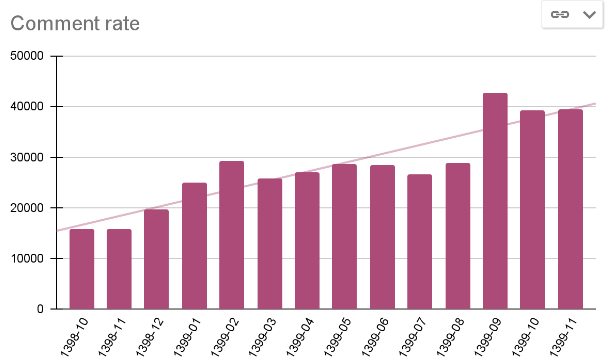
\includegraphics[width=15cm]{figs/comment_rate.png}
\caption{تعداد نظرات در ماه‌های مختلف}\label{}
\label{fig:test}
\end{figure}

در این ماه‌ها، نظرات ثبت شده در دیجی‌کالا از ۱۵ هزار عدد نظر ثبت شده به ۴۰ هزار عدد رسیده است! باید بگوییم که در حال حاضر یعنی در سال ۱۴۰۰، حتی این عدد به ۵۰ هزار هم نزدیک شده است. اینجا بود که فهمیدیم، کارشناس‌ها واحد تیم محتوا دیگر نمی‌توانند به‌صورت دستی، این حجم از نظرات را مدیریت کنند. چون با همان سیستم قبلی باید شدت حدود ۳ برابر کار می‌کردند که این عملا غیر ممکن است!
از نظر ما، تنها راهکار برطرف کردن این چالش، خودکارسازی فرایندها به کمک هوش مصنوعی بود. اما قبل از اینکه، از خودکارسازی و استفاده از قابلیت‌های هوش مصنوعی صحبت کنیم؛ بهتر است که اول نگاهی به سیستم قبلی داشته باشیم

در مدل قبلی، ۹۹ درصد از نظرات توسط کارشناس‌ها مدیریت می‌شد. به‌این‌ترتیب که ۹۶ درصد آن‌ها تایید و ۳ درصد آن‌ها رد می‌شد. سهم هوش مصنوعی در مدیریت این نظرات، فقط یک درصد بود! یعنی فقط یک درصد از کل نظرات ثبت شده در دیجی‌کالا به‌صورت خودکار رد می‌شدند.
برای درک بهتر این موضوع، لازم است تا نگاهی به نمودار زیر بیاندازیم:

\begin{figure}[H]
\centering
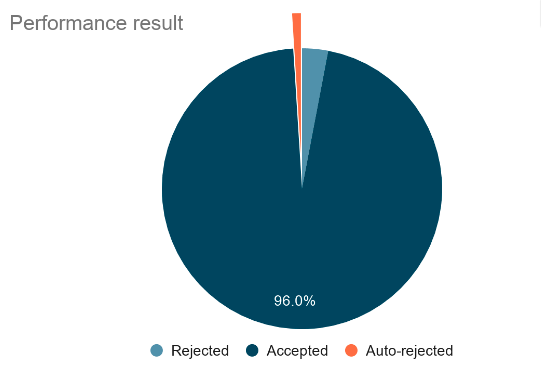
\includegraphics[width=15cm]{figs/performance_result.png}
\caption{سهم مدل قبلی از نظرات}\label{}
\label{fig:test}
\end{figure}

 این مدل، یک شبکه عصبی عمیق بر پایه
 \trans{بلندواژه‌ی کوتاه حافظه}{LSTM}
  است. شاید در ظاهر مدل ناکارآمدی نباشد، اما در کاهش چالش‌ها برای واحد مدیریت نظرات، خیلی هم موثر نبود. چون این مدل فقط می‌توانست بخشی از نظرات را «رد» کند. یعنی قابلیت بررسی نظرات برای «تایید»‌ آن‌ها را نداشت!
جالب است بدانید که باتوجه‌به به استانداردها و سیاست‌های تیم محتوای دیجی‌کالا، فقط ۴ درصد از کل نظرات رد می‌شوند. پس این مدل فقط می‌توانست روی ۴ درصد تاثیرگذار باشد که از این مقدار هم، طبق نمودار بالا، فقط یک درصد از نظرات را تشخیص داده و رد می‌کرد. به همین دلیل سهم چشمگیری در کاهش حجم کاری کارشناسان ایفا نمی‌کرد. پس به مدلی نیاز داشتیم که بتواند علاوه بر رد کردن نظرات، به تایید آن‌ها هم بپردازد.


\قسمت{اهداف تحقیق}
در این پایان‌نامه هدف پیاده‌سازی مدل تجزیه و تحلیل احساسات نظرات دیجی‌کالا است. به همین منظور ابتدا روش‌هایی برای مدیریت تعداد زیاد نظرات به کمک هوش مصنوعی می‌پردازیم و سپس روش خلاقانه‌ای برای تحلیل احساسات نظرات ارائه خواهیم نمود. 
\قسمت{ساختار پایان‌نامه}
در فصل دوم به بررسی مفاهیم اولیه مرتبط با پایان‌نامه پرداخته و گریزی به روش‌های پیشین خواهیم داشت؛ سپس در فصل سوم به تشریح روش تکمیلی و خلاقانه‌ای که از آن در شرکت دیجی‌کالا بهره برده‌ایم، خواهیم پرداخت. در فصل چهارم به بررسی نتایج به دست آمده حاصل از روش خلاقانه پرداخته‌ایم و در نهایت در فصل پنجم کارها و مسیرهای احتمالی پیش رو را تبیین می‌نماییم.